\chapter{Probability and Statistics}

    Before we delve into statistical mechanics, we first have to go through the mathematics on which the subject is built. Before starting this chapter, let us make a few definitions.
    \paragraph{Trial:}A process at the end of which one obtains certain outcomes.
    \paragraph{Event:}Each outcome of a trial.
    \paragraph{Probability:}Measure of likelihood of occurrence of an event.
    There are two ways of asigning a probability to an event. First of these is the statistical probability.
    \paragraph{Statistical Probability:}Probability assigned to events based on relative frequency. Given that an experiment with $N$ trials yields $n_A$ occurrences of event $A$, the \textbf{probability} $P(A)$ of event $A$ occurring is
    \begin{equation}
        P(A) = \lim_{N\to\infty}\frac{n_A}{A}.
    \end{equation}
    In real experiments, it is obvious that one cannot conduct infinitely many trials. However, upon conducting a large amount of experiments one may utilise other methods to produce probabilities.
    
    The second way to assign a probability is the classical probability.
    \paragraph{Classical (A Priori) Probability:}Probability assigned to an event before it takes place, assigning equal likelihood to all outcomes.
\newpage
    \section{Axioms of Probability Theory}
        To define an axiomatic system of a theory of probability, we have to borrow some ideas from set theory. Let us take the die as an example and consider three events $A,B$, and $C$. 
        \begin{itemize}
            \item \textbf{Event A:} An odd number smaller than 4
            \item \textbf{Event B:} An odd number smaller than 2
            \item \textbf{Event S:} Certain event. Any number between 1 and 6.
        \end{itemize}
        \begin{figure}[H]
            \centering
                \tikzset{every picture/.style={line width=0.75pt}} %set default line width to 0.75pt        
                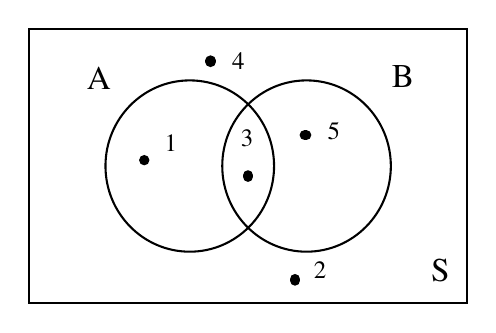
\begin{tikzpicture}[x=0.75pt,y=0.75pt,yscale=-1,xscale=1]
                    %uncomment if require: \path (0,300); %set diagram left start at 0, and has height of 300
                    
                    %Shape: Rectangle [id:dp5602169304393213] 
                    \draw   (100,41.67) -- (311,41.67) -- (311,174) -- (100,174) -- cycle ;
                    %Shape: Ellipse [id:dp4357935586445133] 
                    \draw   (136.98,107.83) .. controls (136.98,85.04) and (155.16,66.57) .. (177.59,66.57) .. controls (200.02,66.57) and (218.21,85.04) .. (218.21,107.83) .. controls (218.21,130.62) and (200.02,149.1) .. (177.59,149.1) .. controls (155.16,149.1) and (136.98,130.62) .. (136.98,107.83) -- cycle ;
                    %Shape: Ellipse [id:dp5865551607027422] 
                    \draw   (193.25,107.83) .. controls (193.25,85.04) and (211.43,66.57) .. (233.86,66.57) .. controls (256.29,66.57) and (274.47,85.04) .. (274.47,107.83) .. controls (274.47,130.62) and (256.29,149.1) .. (233.86,149.1) .. controls (211.43,149.1) and (193.25,130.62) .. (193.25,107.83) -- cycle ;
                    %Shape: Free Drawing [id:dp6682110093205644] 
                    \draw  [line width=3.75] [line join = round][line cap = round] (155.67,105) .. controls (155.67,105) and (155.67,105) .. (155.67,105) ;
                    %Shape: Free Drawing [id:dp2277868619577088] 
                    \draw  [line width=3.75] [line join = round][line cap = round] (205.67,112.33) .. controls (205.67,112.56) and (205.67,112.78) .. (205.67,113) ;
                    %Shape: Free Drawing [id:dp833320635160391] 
                    \draw  [line width=3.75] [line join = round][line cap = round] (233.67,93) .. controls (233.44,93) and (233.22,93) .. (233,93) ;
                    %Shape: Free Drawing [id:dp7574780843900116] 
                    \draw  [line width=3.75] [line join = round][line cap = round] (228.33,162.33) .. controls (228.33,162.56) and (228.33,162.78) .. (228.33,163) ;
                    %Shape: Free Drawing [id:dp7194338325314746] 
                    \draw  [line width=3.75] [line join = round][line cap = round] (187.67,57) .. controls (187.67,57.22) and (187.67,57.44) .. (187.67,57.67) ;
                    
                    % Text Node
                    \draw (126.49,58.57) node [anchor=north west][inner sep=0.75pt]   [align=left] {{\fontfamily{ptm}\selectfont {\large A}}};
                    % Text Node
                    \draw (273.51,57.84) node [anchor=north west][inner sep=0.75pt]   [align=left] {{\fontfamily{ptm}\selectfont {\large B}}};
                    % Text Node
                    \draw (292.39,150.98) node [anchor=north west][inner sep=0.75pt]   [align=left] {{\fontfamily{ptm}\selectfont {\large S}}};
                    % Text Node
                    \draw (164,91.33) node [anchor=north west][inner sep=0.75pt]   [align=left] {{\small {\fontfamily{ptm}\selectfont 1}}};
                    % Text Node
                    \draw (200.67,88.67) node [anchor=north west][inner sep=0.75pt]   [align=left] {{\small {\fontfamily{ptm}\selectfont 3}}};
                    % Text Node
                    \draw (235.86,152.1) node [anchor=north west][inner sep=0.75pt]   [align=left] {{\small {\fontfamily{ptm}\selectfont 2}}};
                    % Text Node
                    \draw (242.53,85.43) node [anchor=north west][inner sep=0.75pt]   [align=left] {{\small {\fontfamily{ptm}\selectfont 5}}};
                    % Text Node
                    \draw (196.53,51.43) node [anchor=north west][inner sep=0.75pt]   [align=left] {{\small {\fontfamily{ptm}\selectfont 4}}};
                \end{tikzpicture}
            \caption{A Venn diagram of events $A$, $B$, and $S$.}
            \label{fig:venndiagram}
        \end{figure}
        Here, we can see that Event $S$ is the whole set of events. If we want to get the Event $A$ OR Event $B$, we have $A\cup B = \{1,3,5\}$ and if we want to get both the Event $A$ AND Event $B$, we have $A\cap B = \{3\}$. \\
        \\
        Now, let us state the axioms of the probability theory.
        \begin{enumerate}
            \item The probability $P(A)$ of an event $A$ is a non-negative number assigned to that event.
            \begin{equation}
                P(A)\geq 0
            \end{equation}
            \item The probability of a certain event is 1.
            \begin{equation}
                P(S) = 1
            \end{equation}
            \item If $A\cap B = \emptyset$, where $\emptyset$ denotes the empty set, then
            \begin{equation}
                P(A+B) = P(A) + P(B)
            \end{equation}
        \end{enumerate}
        Axiom (3) describes the \textbf{mutually exclusive} events: Events that cannot happen at the same time.
        \begin{problem}{Consider a box with 3 green, 5 blue, and 4 red balls. A ball is drawn at random. What is the probability that the ball drawn is either green or blue?}
        bSince there are 12 balls in total we have \[P(G) = \frac{3}{12} \hspace{1cm} P(B) = \frac{5}{12.}\] And since both events cannot happen simultaneously, they are mutually exclusive events and thus \[ P(B+G) = \frac{8}{12} = \frac{2}{3}.\]
        \end{problem}
        \begin{problem}{Two dice are rolled. What is the probability that sum of two numbers is 7?}
           bLet us list all possibilities: $\{2,3,4,5,6,7,8,9,10,11,12\}$. Then, we get $P = 1/N = 1/11$. However, this is a wrong answer simply because the event that the sum of the numbers is 7 depends on the pair of trials. The correct way to count the desired outcomes is:$ \{(1,6),(2,5),(3,4),(4,3),(5,2),(6,1)\}$. Since the total number of pairs is $6^2=36$, we get \[P =6/36 = 1/6.\]
        \end{problem}
        One can note the in Problem 3, not all outcomes are equally likely. So a question is: How does one assign a priori probability to events?
        \paragraph{Principle of Insufficient Reason / Principle of Indifference: }In the absence of any a priori knowledge, we must assume that each relevant outcome $A_i$ must be equally likely.
        \paragraph{Independent Outcomes:} If the probability of both events occurring is the product of single event probabilities then the two events are \textbf{independent} or \textbf{uncorrelated}. 
        \begin{equation}
            P = \prod_i P_i
        \end{equation}
    \section{Counting the Number of Events}
        The simple act of counting the number of ways in which the events can occur leads to the definition of important concepts like arrangements, permutations, and combinations. Let us begin with arrangements. Here, a number of objects is arranged along a line. The number of possible arrangements change depending on the objects that are arranged are similar or not.\\
        \begin{enumerate}
            \item The number of ways of arranging $n$ dissimilar objects in a line is $n!$.
            \item The number of ways of arranging $n$ objects, $p$ of which are identical along a line is $n!/p!$.
        \end{enumerate}
        If we'd like to generalize the second arrangement, if there are $n$ objects $p_1$ of which are one kind, $p_2$ of which are another kind and so on, then the number of ways in which the objects can be arranged along a line is
        
        \begin{equation}
            \frac{n!}{\prod_ip_i!}
        \end{equation}
        
        Now let us consider the permutations. These are the cases where a number of objects are chosen out of a larger set of objects and where one choice is independent of the other. Choosing $r$ objects out of $n$ objects is called the \textbf{permutation} of $r$ out of $n$. We write the number of permutations as
        
        \begin{equation}
            ^nP_r = \frac{n!}{(n-r)!}.
        \end{equation}
        
        Finally, we have the combinations where again $r$ objects are chosen out of $n$ objects but the order of the choice does not matter. Consider 10 pieces of chalk where three are chosen. Then by Equation 3.2.2,
        
        \begin{equation}
            ^{10}P_3 = \frac{10!}{(10-3)!} = \frac{10!}{7!} = 10\times9\times8.
        \end{equation}
        
        Now let us name the chosen chalks as $A,B$, and $C$. Then there are $3!$ orders in which we can select these three chalks. Here, we define the \textbf{combination} as
        
        \begin{equation}
            3!^{10}C_3 = ^{10}P_3.
        \end{equation}
        
        In general, the number of combinations of $r$ objects out of $n$ is
        
        \begin{equation}
            ^nC_r=\frac{n!}{r!(n-r)!}.
        \end{equation}
        
        Now let us define the concept of a box. Upon choosing any amount $r$ objects out of $n$ objects, we put the chosen objects into a box so that they cannot be chosen anymore. Then, another $q$ amount of objects are chosen from what is now $n-r$ objects and again put into a box. This goes on until all the objects are separated into boxes. In general, the number of arrangements for $N$ pieces of objects with $n_i$ in box $i$ is 
        
        \begin{equation}
            W = \frac{N!}{\prod_in_i!}.
            \label{eq:box}
        \end{equation}
        
        Equation (\ref{eq:box}) can be used to work out the total number of ways energy can be arranged between different quantum mechanical states levels in $N$ identical systems where $n_i$ represent the number of times this quantum state is occupied.
    \section{Distributions}
        The outcomes of events are not, in general, uniform. When looking at the statistical data of an experiment, over which one may assign a statistical probability, in a plot of outcomes versus occurrences different shaped plots appear for different cases. These plots are called \textbf{probability distribution functions (PDFs)} or just distributions in short. Let $X$ be a variable that takes on numerical values determined by the outcome of a random experiment. Such variables are called \textbf{random variables}. Random variables can either take discrete values (which are then called \textbf{discrete random variables}) or can lie on a continuous spectra. A probability distribution function $P(X=x)$ express the probability that a random variable $X$ takes on a value $x$. There are two main properties of PDFs.
        \begin{enumerate}
            \item Since the probability is a non-negative value, so must the value of a PDF at a value $x$. \(P(X=x) \geq 0\) \( \forall X\)
            \item The probability that the experiment yields a result is always unity. Thus, the sum of all possible values taken by a PDF must be unity. \(\sum_xP(x)=1\)
        \end{enumerate}

        Rather than looking at the probability of a single outcome, one can also define a function that gives the probability that the outcome is greater than a set amount, i.e. the probability that $X$ is less than or equal to $x_0$. Such functions are called \textbf{cumulative probability functions}.\\
        \\
        In their essence, PDFs are just histograms with continuous PDFs having the limit as the bin size goes to zero or the bin count goes to infinity. Therefore, we can calculate the same important quantities for PDFs just as we can do for histograms.\\
        \\
        Let us consider an experiment where the possible outcomes are binned in a histogram. Here we can describe the results of the experiment using 
        \begin{itemize}
            \item \textbf{Mean:} The arithmetic average of the outcomes. 
            \begin{equation}
                \bar{x} = \frac{1}{N}\sum_i^N x_i
            \end{equation}
            \item \textbf{Median:} The value at the middle in an ordered list of outcomes.
            \item \textbf{Mode:} The outcome that occurs the most often.
        \end{itemize}
        These three measures are called \textbf{central tendency measures}. If the distribution is binned, then the mean is given by
        \begin{equation}
            \bar{x} = \frac{1}{N}\sum_i^Nn_ix_i
            \label{eq:defmean}
        \end{equation}
        where $N$ is the amount of trials and $n_i$ is the number in bin $i$. By defining the statistical probability $p_i = n_i/N$ and taking the limit as $N$ goes to infinity, we can write Equation (\ref{eq:defmean}) as
        \begin{equation}
            \bar{x} = \sum_i^Np_ix_i.
        \end{equation}
        Although the mean value in a PDF provides valuable information, it cannot be used alone to define or make predictions about an experiment. To quantify how much the values deviate from the average we define two quantities. 
        \begin{itemize}
            \item \textbf{Variance:} Average of squared deviations of values from the mean.
            \begin{equation}
                (\Delta x)^2 = \frac{1}{N}\sum_i^N(x_i-\bar{x})^2
            \end{equation}
            \item \textbf{Standard Deviation:} Square root of the variance.
            \begin{equation}
                \Delta x = \sqrt{\frac{1}{N}\sum_i^N(x_i-\bar{x})^2}
            \end{equation}
        \end{itemize}
        Similarly, we can use the sstatistical probability to write the variation as 
        \begin{equation}
            (\Delta x)^2 = \sum_ip_i(x_i-\bar{x})^2.
            \label{eq:stddevdefn}
        \end{equation}
        Although there are several important PDFs that are generally used throughout physics, the most common one is the \textbf{Gaussian / Normal Distribution}. This is due to the \textbf{Central Limit Theorem (CLT)}.
        \begin{theorem}{Central Limit Theorem}
            bUnder appropriate conditions, the distribution of a normalized version of the sample mean converges to a standard normal distribution.
        \end{theorem}
        In general, the appropriate conditions are taken as the cases where the number of samples is larger than 30. If the Gaussian distribution is continuous, it is given by the function
        \begin{equation}
            p(x) = \frac{e^{-(x-\mu)^2/2\sigma^2}}{\sqrt{2\pi}\sigma}.
            \label{eq:gaussian}
        \end{equation}
        This distribution, as suggested by its name, is a Gaussian function and thus is bell-shaped. This is seen in Figure (\ref{fig:gaussian}).
        \begin{figure}[H]
            \centering
            \resizebox{0.75\textwidth}{!}{%
            \begin{tikzpicture}
                  \begin{axis}[
                    width = 17.5cm,
                    height = 7.25cm,
                    xmin = -4.5, xmax = 4.5,
                    ymin = 0,
                    axis x line = bottom, % the * suppresses the arrow tips
                    hide y axis,
                    xtick = {-1,...,1},
                    % xtick = {0},
                    % tick label style = {color=white}, % uncomment this line and change all other
                    % xtick tags to remove x-axis markings
                    xtick align = outside,
                    xticklabels = {
                      $(\bar{x}-\Delta x)$, $\vphantom{(}\bar{x}$, $(\bar{x}+\Delta x)$}, % comment this if uncomment above;
                        %commenting this without uncommenting above makes markings integers
                  ]
                  % This draws the vertical lines
                  \pgfplotsinvokeforeach {-1,0,1} {
                    \draw[black, thick] (axis cs: #1,-1)
                      -- (axis cs: #1,{(1/sqrt(2*pi))*exp((-1/2)*(#1)^2)});
                  }
                        
                  % This draws the main curve
                  \addplot [
                    domain = -4.5:4.5, 
                    samples = 251, 
                    color = red,
                    very thick,
                    name path = dist
                  ]
                  {(1/sqrt(2*pi))*exp((-1/2)*x^2)};

                  \addplot [
                    domain = -1.22:1.22,
                    samples = 3,
                    color = blue,
                    very thick
                  ]
                  {1/(2*sqrt(2*pi))};
                \end{axis}
                \end{tikzpicture}
                }
            \caption{Shape of the Gaussian distribution. The blue line indicates the FWHM.}
            \label{fig:gaussian}
        \end{figure}
\newpage
        Now, note that the maximum value of this function is at $x=\mu$. Since this value has to be the mean of the distribution, we get $\mu = \bar{x}$. An important interval of outcomes is the \textbf{Full Width at Half Maximum (FWHM)}. This interval is the width of the "bell" where the height is at the half of the maximum height. To calculate this let $x=\bar{x}$ since we know that $P(\bar{x})$ is the maximum value of the distribution.
        \begin{equation}
            p(\bar{x}) = \frac{e^{-(\bar{x}-\bar{x})^2/2\sigma^2}}{\sigma\sqrt{2\pi}} = \frac{1}{\sigma\sqrt{2\pi}} \Rightarrow \text{HM} = \frac{1}{2\sqrt{2\pi}\sigma}
        \end{equation}
        Since the distribution is symmetric around $\bar{x}$, there will be two values of $p(x)$ corresponding to $x=x_\text{HM}$. 
        \begin{equation}
            p(x_\text{HM}) = HM \Rightarrow \frac{e^{-(x_1-\bar{x})^2/2\sigma^2}}{\sqrt{2\pi}\sigma} = \frac{1}{2\sqrt{2\pi}\sigma} \Rightarrow \frac{(x_1-\bar{x})^2}{2\sigma^2} = \ln2 
        \end{equation}
        \begin{equation}
            (x_\text{HM}-\bar{x})^2 = 2\sigma^2\ln2
        \end{equation}
        \begin{equation}
            \therefore x_\text{HM} = \mp\sqrt{2\ln2}\sigma+\bar{x}
        \end{equation}
        This is the full width at half maximum.
        Recall the second property of the PDFs that $\sigma_xP(x)=1$. However, this may not be the case in general. This property is called the \textbf{normalization} and if a PDF is not normalized at the beginning. It has to be normalized before solving any questions. At the continuous limit, the discrete summation becomes an integral.
        
        \begin{equation}
            \int_\mathcal{\tau}P(x)d\tau = \frac{1}{\sqrt{2\pi}\sigma}\int_{-\infty}^{\infty}dxe^{-(x-\bar{x})^2/2\Delta x^2} \notag 
        \end{equation}
        \begin{equation}
            = \frac{1}{\sqrt{2\pi}\sigma}\sqrt{2\sigma^2\pi} = 1
        \end{equation}
        Therefore, the definition of the normal distribution given in Equation (\ref{eq:gaussian}) is already normalized. Finally, let us now calculate the standard deviation in the normal distribution. For a continuous distribution, Equation (\ref{eq:stddevdefn}) becomes
        \begin{equation}
            (\Delta x)^2=\int_{-\infty}^\infty p(x)(x-\bar{x})^2 dx.
        \end{equation}
        Then,
        \begin{equation}
            (\Delta x)^2 = \frac{1}{\sigma\sqrt{2\pi}}\int_{-\infty}^{\infty}\exp\lrp{-\frac{(x-\bar{x})^2}{2\sigma^2}}(x-\bar{x})^2dx
        \end{equation}

        Let us define a variable $\alpha$ and do a u-substitution.
        \begin{equation}
            \alpha = \frac{1}{2\sigma^2} \hspace{1cm} u=x-\bar{x}\Rightarrow du=dx
        \end{equation}
        This gives us
        \begin{equation}
            (\Delta x)^2 = \frac{1}{\sigma\sqrt{2\pi}}\int_{-\infty}^\infty e^{-\alpha u^2}u^2du. = -\frac{1}{\sigma\sqrt{2\pi}}\periv{}{\alpha}\int_{-\infty}^\infty e^{-\alpha u^2}du
        \end{equation}
        This is the Gaussian integral that we know how to solve. 
        \begin{equation}
            (\Delta x)^2 = -\frac{1}{\sigma\sqrt{2\pi}}\periv{}{\alpha}\lrp{\sqfrac{\pi}{\alpha}} = -\frac{1}{\sigma\sqrt{2}}\periv{\alpha^{-1/2}}{\alpha} = \frac{1}{2\sqrt{2}\sigma}\alpha^{-3/2}
        \end{equation}
        Substituting the $\alpha$ back,
        \begin{equation}
            (\Delta x)^2 = \frac{1}{2\sqrt{2}\sigma}\lrp{\frac{1}{2\sigma^2}}^{-3/2} = \frac{\sqrt{8\sigma^6}}{\sqrt{8}\sigma} = \sigma^2.
        \end{equation}
        Thus, we see that $\Delta x = \sigma$. Then, we can write the Gaussian distribution as
        \begin{equation}
            p(x) = \frac{\exp\lrp{-\frac{(x-\bar{x})^2}{2(\Delta x)^2}}}{\sqrt{2\pi}\Delta x}.
        \end{equation}
        